\documentclass[12pt]{article}
\usepackage{geometry}
\geometry{a4paper, total= {170mm,250mm}}
\title{HomeWork 9}
\author{Maedeh Karkhaneh Yousefi - 98100991}
\usepackage{float}
\usepackage{graphicx}
\usepackage{amsmath}
\usepackage{subcaption}
\begin{document}
\maketitle
\part*{1. First Order ODE}
RC circuit equation should be solved using the Euler algorithm for this part. 
The Euler algorithm: 
\begin{gather*}
v_{n+1} = v_{n} + a_{n} \Delta t \\
x_{n+1} = x_{n} + v_{n} \Delta t
\end{gather*}
The equation that should be solved is: 
\begin{gather*}
\dot{q}= \dfrac{V_{0}}{R} - \dfrac{q}{RC}
\end{gather*}
We put the following form for the function in code:
\begin{gather*}
\dot{q} = q_{0}(1-q)/ RC\ ,\ q_{0}\equiv CV_{0}
\end{gather*}
The increment of the global error with changing the step values is also shown for the Euler algorithm.
\paragraph*{} At last, I've used the following algorithm, which was mentioned in class, to solve the problem. The instability is obvious from the plot. 
\begin{gather*}
x_{n+1} = x_{n-1} + 2\Delta t \dot{x} (t_{n}, x_{n})
\end{gather*}
\begin{figure}[H]
	\centering
	\begin{subfigure}[t]{0.8\textwidth}
		\includegraphics[width=\textwidth]{Euler_compare.pdf}
		\label{fig:mesh1.1}
		\caption{}
	\end{subfigure}\par\bigskip 
	\begin{subfigure}[t]{0.8\textwidth}
		\includegraphics[width=\textwidth]{Euler_Error.pdf}
		\label{fig:mesh1.2}
		\caption{}
	\end{subfigure}
	\label{fig:mesh1}
	\caption{Solving the RC circuit equation using the Euler algorithm. the time range is between 0.0 to 5.0 seconds. step equals to 0.01.}
\end{figure}
\begin{figure}[H]
	\centering
	\includegraphics[width=\textwidth]{Instability.pdf}
	\label{fig:mesh2}
	\caption{Instability plot of RC circuit equation for the given algorithm. Step size= 0.08. time ranging from 0.0 to 5.0 seconds. }
\end{figure}
\part*{2. Second Order ODE}
Simple Harmonic Oscillator's equation has been solved with the Euler Method and the following algorithms and the comparison plots and the phase space plots are followed. 
\paragraph*{\textbf{Euler-Cromer Algorithm : }}
\begin{gather*}
v_{n+1} = v_{n} + a_{n} \Delta t \\
x_{n+1} = x_{n} + v_{n+1} \Delta t
\end{gather*}
\paragraph*{\textbf{Verlet Algorithm : }}
\begin{gather*}
x_{n+1} = 2x_{n} - x_{n-1} + a_{n} (\Delta t)^{2}\\
v_{n+1} = \dfrac{x_{n+1} - x_{n}}{h}
\end{gather*}
\paragraph*{\textbf{Velocity Verlet Algorithm : }}
\begin{gather*}
x_{n+1} = 2x_{n} + v_{n} \Delta t + \dfrac{1}{2}a_{n} (\Delta t)^{2}\\
v_{n+1} = v_{n} + \dfrac{1}{2} (a_{n+1} + a_{n}) \Delta t
\end{gather*}
\paragraph*{}SHM equation: 
\begin{gather*}
\ddot{x}= -\omega x
\end{gather*}
\begin{figure}[H]
	\centering
	\includegraphics[width=\textwidth]{SHM_Euler_comparison.pdf}
	\label{fig:mesh}
	\caption{Place-Time and Velocity-Time Plots. Comparison between Euler method's and the analytic solution for SHM (n=5) and time range between 0.0 and 8.0 seconds. $x_{initial} = 1.0$ and $v_{initial} = 0.0$.}
\end{figure}
\begin{figure}[H]
	\centering
	\begin{subfigure}{0.8\textwidth}
		\includegraphics[width=\textwidth]{SHM_v_comparison.pdf}
		\label{fig:mesh4.2}
		\caption{}
	\end{subfigure}
		\begin{subfigure}{0.8\textwidth}\par\bigskip 
		\includegraphics[width=\textwidth]{SHM_x_comparison.pdf}
		\label{fig:mesh4.2}
		\caption{}
	\end{subfigure}
	\label{fig:mesh}
	\caption{Place-Time and Velocity-Time Plots. Time range between 0.0 and 31.0 seconds, n=5, $x_{initial} = 1.0$ and $v_{initial} = 0.0$. }
\end{figure}
\begin{figure}[H]
	\centering
	\begin{subfigure}{0.8\textwidth}
		\includegraphics[width=\textwidth]{SHM_Euler_PhaseSpace.pdf}
		\label{fig:mesh5.2}
		\caption{}
	\end{subfigure}
		\begin{subfigure}{0.8\textwidth}\par\bigskip 
		\includegraphics[width=\textwidth]{SHM_All_PhaseSpace.pdf}
		\label{fig:mesh5.2}
		\caption{}
	\end{subfigure}
	\label{fig:mesh}
	\caption{Phase space plots. n=5, $x_{initial} = 1.0$ and $v_{initial} = 0.0$.}
\end{figure}
\part*{3. Bifurcation}
Mathematically the logistic map is written as:
\begin{gather*}
x_{n+1} = 4rx_{n}(1-x)
\end{gather*}
By using this function, the bifurcation can be seen from the plot. I created a range of r values in between 0.0 and 1.0, then for each r, I generated an array of $x_{0}$ values in range (0.0, 1.0). These values are passed to the function, and the final x values will be returned after a repetition of $10^{4}$.
\begin{figure}[H]
	\centering
	\begin{subfigure}{0.6\textwidth}
		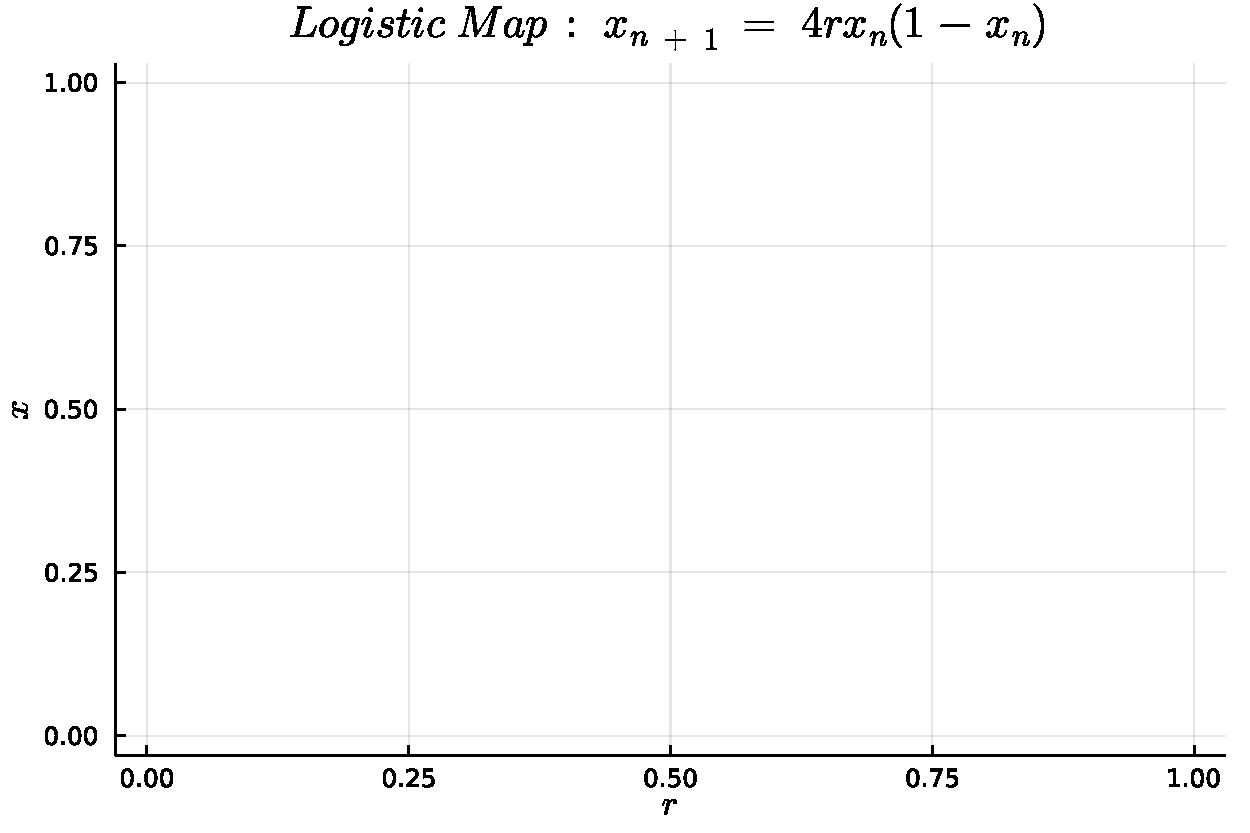
\includegraphics[width=\textwidth]{Bifurcation.pdf}
		\label{fig:mesh5.2}
		\caption{}
	\end{subfigure}
		\begin{subfigure}{0.6\textwidth}\par\bigskip 
		\includegraphics[width=\textwidth]{Zoomed_Bifurcation.pdf}
		\label{fig:mesh5.2}
		\caption{}
	\end{subfigure}
	\label{fig:mesh}
	\caption{Bifurcation plots. $\Delta r= 10^{-4}$, $0.0<r<1.0$, $n=10^{4}$. }
\end{figure}
\paragraph*{\textbf{Feigenbaum constants}}
\begin{gather*}
\sigma = \lim_{n\rightarrow \infty} \dfrac{r(d_{n})-r(d_{n-1})}{r(d_{n+1})-r(d_{n})} = 4.6692
\end{gather*}
And I acquired the value $\sigma \sim 4.627451$, for step= $10^{-4}$ and n = $10^4$.
\begin{gather*}
\alpha = \lim_{i\rightarrow \infty} \dfrac{L_{i-1}}{L_{i}} = 2.502907
\end{gather*}
And I acquired the value $\alpha \sim 1.5294$, for step= $10^{-4}$ and n = $10^4$.
\end{document}